\documentclass{article}
\usepackage{amsmath, tcolorbox, sfmath, enumerate, pgfplots, multicol}
\renewcommand{\familydefault}{\sfdefault}
\pgfplotsset{compat=newest}
\tikzset{>=stealth}
\usepackage[top = 0.25in, bottom = 0.25in, left = 1.25in, right = 1.25in]{geometry}
\pagestyle{empty}
\raggedright

\newcounter{example}[section]
\newenvironment{example}[1][]{\refstepcounter{example}\par\medskip
   {\color{red}\textbf{Example~\theexample. #1}}}{\medskip}

\begin{document}

\section*{Average Rate of Change}

\begin{tcolorbox}[colframe=orange!70!white, coltitle=black, title=\textbf{Summary}]
\begin{enumerate}
    \item The slope-intercept form of the equation of a line is $y = mx + b$.
    \item Slope represents variable costs; $y$-intercept represents fixed costs.
    \item The average rate of change measures the slope of the line connecting 2 points on a graph.
\end{enumerate}
\end{tcolorbox}
\vspace{0.5in}

\subsection*{Slope-Intercept Form}

Recall that the slope of a line connecting 2 points is  \newline\\
\begin{minipage}{0.2\textwidth}
\[
m = \frac{\text{Rise}}{\text{Run}} = \frac{y_2-y_1}{x_2-x_1}
\]
\end{minipage}
\hfill 
\begin{minipage}{0.4\textwidth}
\begin{tikzpicture}[scale=0.7]
\begin{axis}
[axis lines = middle, xmin = -5.5, xmax = 5.5, ymin = -5.5, ymax = 5.5, ticks = {none}]
\coordinate (A) at (-3,-3);
\addplot [mark = *, only marks, color=blue] coordinates {(-3,-3) (2,2)};
\draw [color=blue, thick] (axis cs: -3,-3) -- (axis cs: 2,2);
\draw [color=red] (axis cs: -3,-3) -- (axis cs: 2,-3) node [midway, below] {Run};
\draw [color=violet] (axis cs: 2,-3) -- (2,2) node [midway, right] {Rise};
\end{axis}
\end{tikzpicture}
\end{minipage}  \hfill 
\vspace{0.5in}

We often write the equation of a line in \textbf{slope-intercept form}: $y = mx+b$, where $b$ is the $y$-intercept.  

\begin{itemize}
    \item The $y$-intercept can be thought of as the \textbf{fixed cost} of doing business (cost no matter what)
    \item The slope can be thought of as the \textbf{variable cost} (cost based on how much is produced).
\end{itemize}
\vspace{0.5in}

\begin{example}
A local company manufactures goods with weekly fixed costs of \$6,000 and variable costs of \$4.55 per item. 
\begin{enumerate}[(a)]
    \item Determine the linear cost function $C(x)$ and interpret $C(1500)$ \vfill 
    \item At 1500 per week production level, what is the cost of manufacturing the 1501st item? (\emph{Note}: This is called the \textbf{marginal cost}) \vfill 
\end{enumerate}
\end{example}

\newpage 

\subsection*{Average Rate of Change}

The {\color{blue}\textbf{average rate of change}} over an interval $[a,b]$ of a function is the slope of the line connecting the endpoints of the interval.  
\[
\frac{\Delta f}{\Delta x} = \frac{f(b)-f(a)}{b-a}
\]


\begin{center}
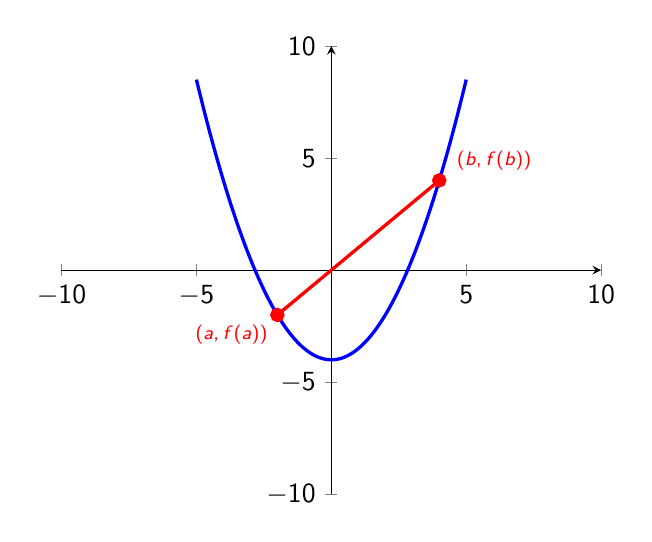
\begin{tikzpicture}
\begin{axis}[
axis lines = middle,
xmin = -10, xmax = 10,
ymin = -10, ymax = 10,
]
\addplot[blue,very thick,samples=200,smooth] {0.5*x^2-4};
\addplot[mark=*, red, very thick] coordinates {(-2,-2) (4,4)};
\node at (axis cs: -2,-2) [below left, red] {\scriptsize $(a,f(a))$};
\node at (axis cs: 4,4) [above right, red, xshift=0.1cm] {\scriptsize $(b,f(b))$};
\end{axis}
\end{tikzpicture}
\end{center}
\vspace{1in} 

\begin{example} 
Find the average rate of change for each.  
\begin{enumerate}[(a)]
    \item $f(x) = 3x - 7 \qquad [2,5]$    \vfill 
    \item $f(x) = 2x^2 - 5x + 4 \qquad [-2, 2]$ \vfill 
\end{enumerate}
\end{example}

\newpage 

\begin{example} 
Find the average rate of change of $f(x) = x^2 + 4x - 1$ over each interval.  
\begin{enumerate}[(a)]
    \item $[3, \, 3.01]$    \vfill 
    \item $[3, \, 3.001]$   \vfill 
    \item $[3, \, 3.0001]$  \vfill 
    \item Do the outputs get closer and closer to a value as the inputs get closer together? If so, what is that value?  \vfill 
\end{enumerate}
\end{example}


\end{document}
